\chapter{Processmodeller}\label{ch:processmodeller}

\section{Den agile metode}
I slut 90’erne blev den agile metode udviklet\cite{Sommerville}. Den blev udviklet som modsvar på den utilfredshed der var med den daværende fremgangsmetode til udvikling af softwaresystemer. Før den agile metode blev indført, var den generelle overbevisning, at den bedste måde at opnå bedst mulig software på, var ved at planlægge det forsigtigt\cite{Sommerville}. Dette syn på udviklingsmetoden kom fra software ingeniør samfundet, som for det meste udviklede software i store teams der arbejdede for forskellige firmaer. Meget af dette software blev brugt til store systemer, så som flysystemer eller til systemer til staten. Derfor krævede processen meget detaljeret planlægning på forhånd, og mere tid blev sat af til planlægning af hvordan systemet skulle være designet end selve udviklingsprocessen eller test\cite{Sommerville}.
Det så ud til, at denne udviklingsmetode virkede fint når det gjaldt udvikling af software til store firmaer, men angående de mindre firmaer eller små forretninger ville den tunge planlægningsmetode ikke altid være den optimale udviklingsmetode. Med den nye metode, fokuserede man på software og hvordan løsningen og designet kan ændre sig efterhånden som man bliver klogere på problemerne der skal løses, i stedet for selve designet og dokumentationen af systemet. Denne fremgangsmåde var nemmere, når det kom til mindre systemer, da udviklingsmetoden og kravenede hurtigt ændrede sig gennem processen\cite{Sommerville}. 
Så, utilfredsheden med den tunge planlægningsmetode ledte til udviklingen af agile metoder, så som eXtreme Programming og Scrum.


\textbf{Hvad er den agile metode så?}

\begin{figure}
    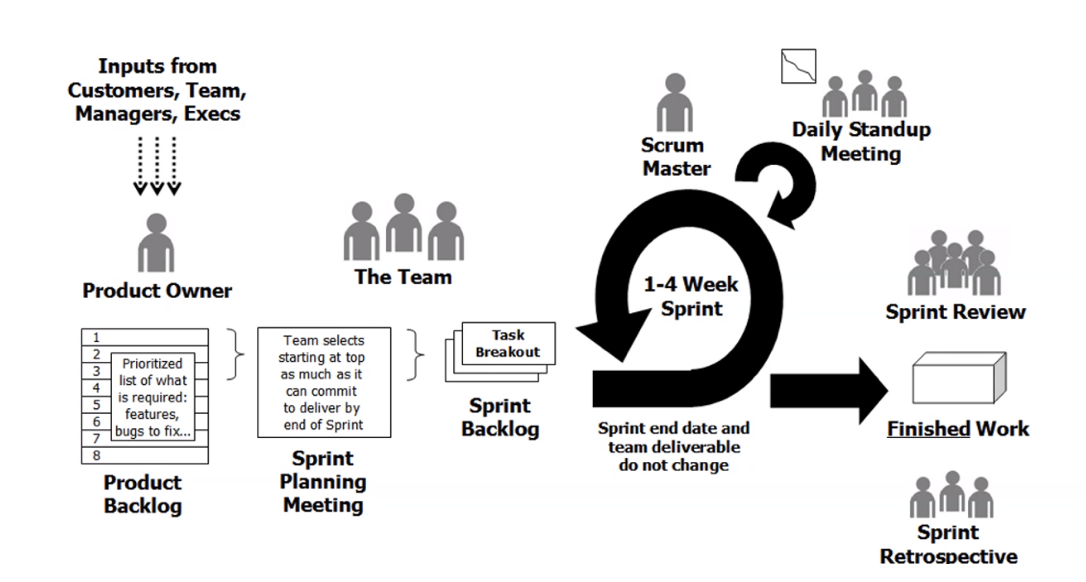
\includegraphics[width=\linewidth]{figures/AgileMetoder.png}
    \caption{Den Agile metode}
    \label{fig:Agil}
\end{figure}

Agile metoder er Rapid software udvikling, det er metoder som er designet til at producere software der ikke bare er blevet produceret hurtigt, men nyttigt\cite{Sommerville}.  Når det gælder agile metoder, er kunderne en del af udviklingsprocessen. Dette kommer i form af de små increments der konstant bliver udviklet og frigjort til kunden. Dette skaber en hurtig feedback tilbage til teamet, så teamet ved hvad der skal forbedres, eller hvis der sker nye forandringer ift. krav. Dette betyder, at teamet gerne skal have feedback hurtigst muligt, og derfor minimerer vi dokumentation (som også er en af målene for agile metoder) og sætter i stedet fokus på informativ kommunikation. Ved plan-dreven udvikling sker kommunikationen mellem stages og med formal dokumentation. De to udviklingsmetoder behøves ikke skilles fra hinanden fuldstændigt, agile metoder kan sagtens benyttes med plan-driven. Agile metoder har været succesfulde for to udviklings strategier;
For det første har agile metoder været succesfulde, når det gælder både lille til medium produktstørrelse, og at stort set alle software produkter og applikationer er udviklet ved brug af en agile tilgang.
For det andet har agile metoder været specielt fordelagtige, eftersom kunden også nu har en vigtig rolle, og deltager i udviklingsprocessen. Derudover er der også få eksterne interessenter, der har indflydelse på softwaren\cite{Sommerville}. 
Givet disse situationer, har agile metoder fungeret fordelagtigt. Grunden er, at kommunikationen mellem interessenter er konstant og uformel. Udover, er softwaret ikke påvirket af en masse tidligere stillet faste krav.

Tidligere blev det nævnt, at agile metoder ikke altid har været mainstream-metoden for softwareudvikling. En af de første populære udviklingsmetoder var The Waterfall Model.

\section{The Waterfall Model}
De første software udviklingsmodeller omhandlede en proces, der bestod af et antal faser, som repræsenterede hvordan udviklingen af software skulle foregå\cite{Sommerville}. 

\begin{figure}
    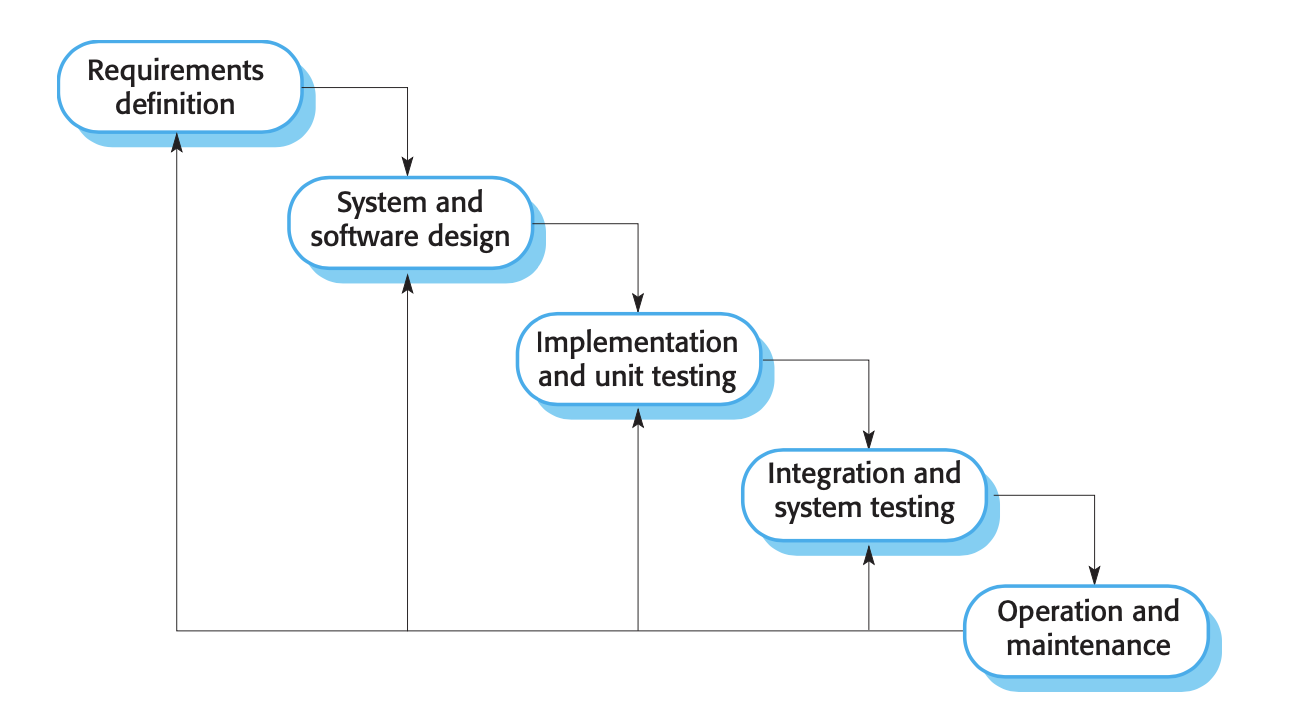
\includegraphics[width=\linewidth]{figures/waterfall_model.png}
    \caption{The Waterfall Model}
    \label{fig:waterfall}
\end{figure}

På figur \ref{fig:waterfall} ses det, at processen har en struktur som afspejler et vandfald, og herfra kommer navnet for The Waterfall Model. Princippet bag modellen er, at teamet planlægger alle aktiviteterne fremadrettet , før udviklingen af softwaren begynder. Herunder ses det at vandfaldsmodellens faser reflekterer de forskellige aktiviteter i traditionel software udvikling.\cite{Sommerville} 
\begin{itemize}
    \item Kravanalyse og definition
    \item System og software design
    \item Implementation og unit tests
    \item Integration og system tests
    \item Kontrol og vedligeholdelse 
\end{itemize}

Ved brug af vandfaldsmodellen, bør man ikke gå videre til næste fase, før den tidligere fase er færdiggjort og dokumenteret. Desuden går man heller ikke tilbage til en tidligere fase for at rette eller ændre nogle beslutninger, hvilket betyder man ofte kan blive låst fast på en dårligere løsning. Problemet ved at gå til software udvikling med denne model, er at gennem udviklingen af et helt projekt vil der altid være et tidligere problem at identificere. Hvad der menes med dette er, at hvis f.eks et team der er i gang med design, vil hurtigt identificere problemer med krav, da det ofte ikke stemmer overens. Til gengæld, vil denne ikke være dårlig for hardware udvikling. Så, nyt information vil altid komme frem, i hver aktivitet. Det betyder, at hvis noget viser sig at være for et kompleks at lave, uden feedback fra kunden, kan der være store forsinkelser i software designet. Dette kan lede til et dårligt design og et halvfærdigt produkt.\cite{Sommerville} 

\section{Metode Valg}

Nu hvor 2 metoder er kort beskrevet, kan gruppen vurderer, om der skal udvikles i vandfaldsmetoden eller en agil metode. Før dette, er det vigtigt at pointere, at gruppen har en begrænset tidsperiode på lidt over 2 måneder til at færdiggøre projektet, som omhandler en web-applikation og en konsol applikation.

Eftersom teamet kun er på 4 personer og målet med projektet er en relativ lille applikation, som skal udvikles, er det besluttet, at applikationen bliver udviklet med agile metoder. Dette er i sig selv ikke grund nok, for at vælge netop det agile over vandfaldsmetoden. Derfor, er det vigtigt at opveje begge metoder. Dette vil hjælpe med bedre at forstå, hvorfor agile metoder fordelagtigt kan vælges over vandfaldsmetoden, specielt gældende dette projekt. Et af de fundamentale grundlag for at vælge agil metode imodsætning til vandfalds, er fordi applikationen er et socialt medie, som operer på cloud-baseret-software eller bedre kendt som software as a service (saas). Saas er en metode, hvori software tillader dataens tilgængelighed til alle enheder med internet adgang og en web browser.\cite{Sommerville} Saas modeller vil aldrig virke med vandfalds baseret udvikling, da det aldrig kan blive færdiggjort, fordi det nettop kræver konstant vedligeholdelse og opdateringer.

Som nævnt tidligere, og beskrevet i Software Engineering af Ian Sommer, så benyttes agile metoder i stort set al software udvikling nu om dage, samt er de fleste apps udviklet ved brug af agile tilgange\cite{Sommerville}.  Kunden for dette projekt er ikke en ekstern kunde heller, men teamet selv, som også er involveret i udviklingen af softwaren og derfor har noget at sige ift. hvordan systemet skal se ud. I denne situation, hvor kunden er selve teamet, er det muligt at have en konstant kommunikation mellem kunden, projektlederen og udviklingsteamet. Siden kunden er teamet selv, vil der være mere feedback gennem processen, med mere præcise krav til systemet og hvordan det skal bruges. Ulempen kan være at systemets brugerflade kan blive indforstået og ikke intuitivt for nye brugere. Teamet er et lille team, og med konstant feedback vil det være nemmere at implementere konstante ændringer i kravene og softwaren til systemet. Dette skulle gerne gøres, uden at gå tilbage og lave dokumenterende ændringer, før en ændring i softwaren kan indføres. Så med den agile model kan teamet hurtigt justere systemet til kundes behov. Nå det så er sagt, kan man konkludere, at den agile tilgang vil være den mest optimale tilgang, for dette projekt.

Med en beslutning om at tage den agile tilgang til projektet, skal der nu tages i betragtning hvilke udviklingsværktøjer, der skal benyttes for at skabe det bedst mulige flow for gruppen. Disse udviklingsværktøjer vil der tages hånd om i næste afsnit, som omhandler Scrum, Extreme Programming (XP) og Kanban.
